\documentclass[a4paper, 12pt]{report}
\usepackage{graphicx}
\usepackage{amsmath, amsthm, amssymb}
\usepackage{enumerate}
\usepackage{hyperref}
\usepackage{caption}
\usepackage[normalem]{ulem}
\usepackage{pdfpages}
\usepackage[toc,page]{appendix}

%%% blank footnote
\newcommand\blfootnote[1]{
	\begingroup
	\renewcommand\thefootnote{}\footnote{#1}
	\addtocounter{footnote}{-1}
	\endgroup
}
%%%

%%% prevent hyphenation
\tolerance=1
\emergencystretch=\maxdimen
\hyphenpenalty=10000
\hbadness=10000
%%%

%%% minimize
\DeclareMathOperator*{\minimize}{minimize}
%%%


\title{Notes\\
\large Machine Learning by Andrew Ng on Coursera}
\author{Sparsh Jain}
\date{\today}

\begin{document}

\maketitle
\tableofcontents
% \listoffigures
% \listoftables

\chapter{Introduction}
\emph{Machine learning} (task, experience, performance) can be classified into
\emph{Supervised} and \emph{Unsupervised} learning.

\section{Supervised Learning}
Supervised learning can be basically classified into \emph{Regression} and
\emph{Classification} problems.

\subsection{Regression Problem}
Regression problems work loosely on continuous range of outputs.

\subsection{Classification Problems}
Classification problems work loosely on discrete range of outputs.

\section{Unsupervised Learning}
An example is \emph{Clustering Problem}.

\blfootnote{Check \autoref{lecture1} for more details.}

\chapter{Linear Regression with One Variable}

\section{Notations}
\begin{align*}
	m                  & = \text{number of training examples}             \\
	x\text{'s}         & = \text{`input' variables / features}            \\
	y\text{'s}         & = \text{`output' variables / `target' variables} \\
	(x, y)             & = \text{single training example}                 \\
	(x^{(i)}, y^{(i)}) & = i^{th} \  \text{example}                       \\
\end{align*}

\section{Supervised Learning}
We have a data set (\emph{Training Set}).

Training Set $\rightarrow$ Learning Algorithm $\rightarrow$ $h$ (\emph{hypothesis},
a function $X \to Y$)

\subsection*{To Represent \texorpdfstring{$h$}{}}
\begin{equation*}
	h_\theta(x) = \theta_0 + \theta_1x
\end{equation*}

\subsection*{Cost}
\begin{equation*}
	\minimize_{\theta_0,\ \theta_1} \frac{1}{2m}\sum_1^m(h_\theta(x) - y)^2
\end{equation*}
\subsubsection*{Cost Function}
Squared Error Cost Function
\begin{equation*}
	J(\theta_0, \theta_1) = \frac{1}{2m}\sum_1^m(h_\theta(x) - y)^2
\end{equation*}
\subsection*{}
\begin{equation*}
	\minimize_{\theta_0,\ \theta_1} J(\theta_0, \theta_1)
\end{equation*}

\section{Gradient Descent}
Finds local optimum:
\begin{enumerate}
	\item Start with some value
	\item Get closer to optimum
\end{enumerate}

\subsection*{Algorithm}
\begin{equation*}
	\theta_j := \theta_j - \alpha\frac{\partial}{\partial\theta_j}J(\theta) \ \forall j
\end{equation*}

where $\alpha$ = learning rate

\subsubsection*{Important!}
Simultaneous Update!
\begin{align*}
	temp_j   & := \theta_j - \alpha\frac{\partial}{\partial\theta_j}J(\theta) \ \forall j \\
	\theta_j & := temp_j \ \forall j
\end{align*}

\section{Gradient Descent for Linear Regression}
Cost function for linear regression is convex!

\emph{Batch Gradient Descent}: Each step of gradient descent uses all training examples.

\blfootnote{Check \autoref{lecture2} for more details.}

\begin{appendices}
	\chapter{Lecture 1} \label{lecture1}
	
\includepdf[pages=-, width=0.9\textwidth]{lecture_pdf/Lecture1.pdf}
	\chapter{Lecture 2} \label{lecture2}
	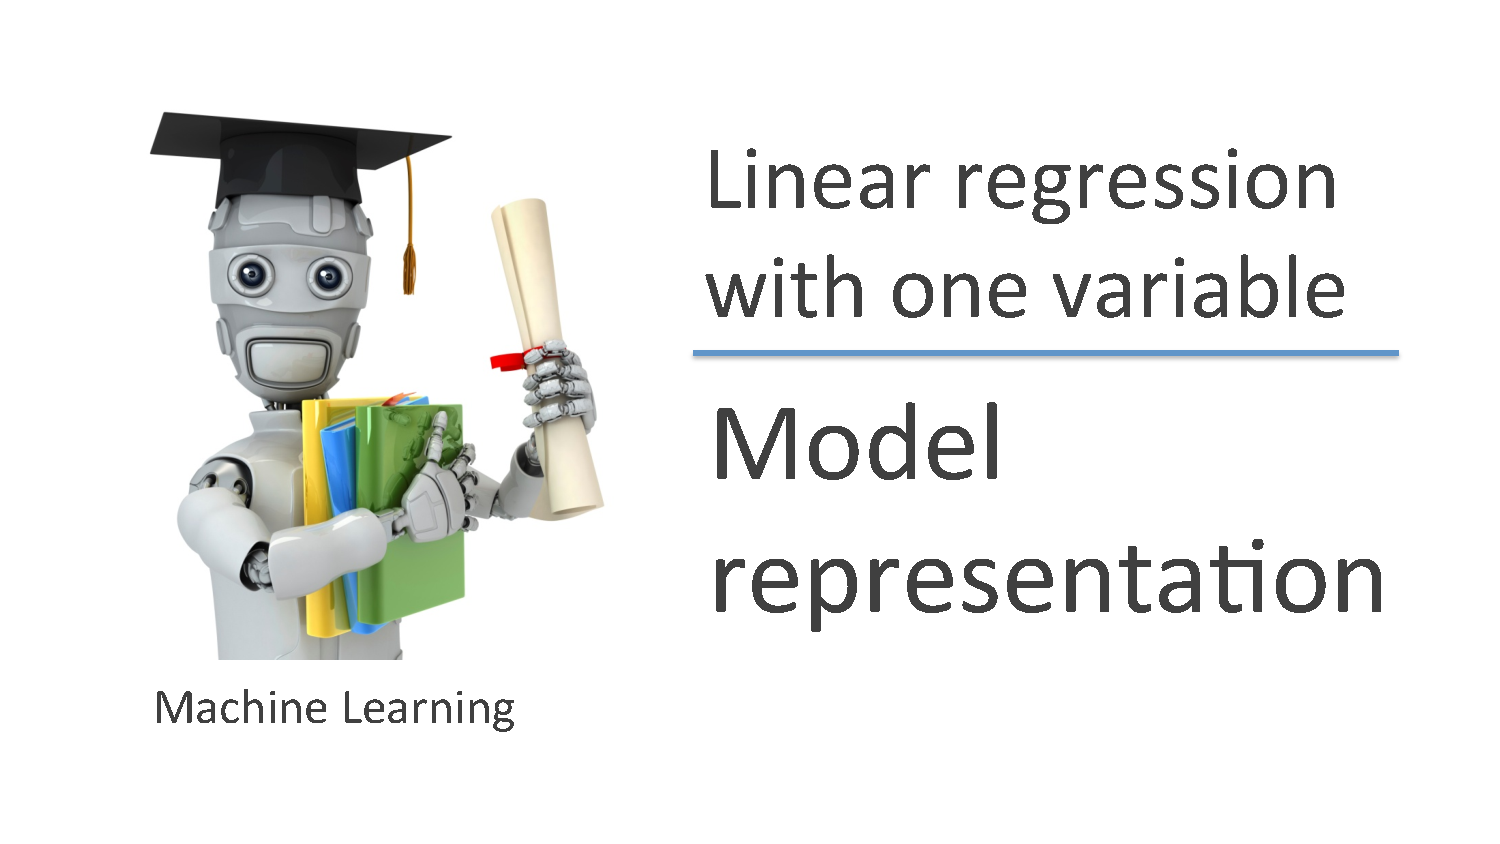
\includepdf[pages=-, width=0.9\textwidth]{lecture_pdf/Lecture2.pdf}
\end{appendices}

\end{document}